% arara: xelatex
% arara: biber
% arara: xelatex: { synctex: true }

\documentclass[12pt,a4paper,oneside,final]{report}

\usepackage{tabularx}

\usepackage{polyglossia}
\setmainlanguage[numerals=cyrillic]{russian}
\setotherlanguages{english}
\usepackage{csquotes}

\usepackage{xunicode}
% some extra unicode support
%\usepackage[utf8x]{inputenc}
\usepackage{xltxtra}
% \XeLaTeX macro
\usepackage{fontspec}
\defaultfontfeatures{Ligatures=TeX}

%\setromanfont{Charis SIL}
%\setsansfont{Liberation Sans}
%\setmonofont{PT Mono}
%\setmainfont{Liberation Serif} % this allows to use sans-serif as default font

\usepackage{ifplatform}

% \ifwindows
\newfontfamily{\cyrillicfont}{Times New Roman}
\setmainfont{Times New Roman}
\newfontfamily{\cyrillicfonttt}{Courier New}
\setmonofont{Courier New}
% \else
%   \setmainfont{Linux Libertine O}
%   \setsansfont{Linux Biolinum O}
%   \setmonofont[SmallCapsFont={Latin Modern Mono Caps}]{Latin Modern Mono Light}
% \fi

%нумерация справа и колонтитулы справа вверху
\usepackage{fancyhdr}
\usepackage[a4paper,left=30mm,right=15mm,top=20mm,bottom=20mm,bindingoffset=0cm]{geometry}
%

\usepackage{amsfonts}
\usepackage{amssymb}
\usepackage{amsmath}
\usepackage{amsthm}

\usepackage{calc}
\usepackage{ifthen}
\usepackage{graphicx}
\usepackage{array}
\usepackage{pdfpages}
\usepackage{longtable}
\usepackage{multirow}
\usepackage{indentfirst}
\usepackage[unicode=true]{hyperref}
\usepackage{color}
\usepackage{pgf}
\usepackage{pstheorems}
\usepackage{titling}
\usepackage{enumitem}

% Настройка списков (без лишних вертикальных отступов)
\usepackage{paralist}
\setdefaultenum{1.}{1.}{1.}{1.}
\setdefaultitem{--}{}{}{}
%\setlength\itemsep{-1em}
\let\itemize\compactitem
\let\enditemize\endcompactitem
\let\enumerate\compactenum
\let\endenumerate\endcompactenum
\let\description\compactdesc
\let\enddescription\endcompactdesc
\pltopsep=\smallskipamount
\plitemsep=0pt
\plparsep=0pt
% Команда для отмены разрыва страниц перед списками
\makeatletter 
\newcommand\mynobreakpar{\par\nobreak\@afterheading} 
\makeatother
%%%%%%

\usepackage[singlelinecheck=false,labelsep=endash]{caption}
\captionsetup[table]{justification=justified}
\captionsetup[figure]{justification=justified,name=Рисунок,singlelinecheck=on,font=onehalfspacing}

\usepackage{titlesec}
\titleformat{\chapter}[block]{\centering\normalfont\Large\bfseries}{\thechapter.}{1ex}{}{}
\titlespacing{\chapter}{0pt}{0em}{2em}

\titleformat{\section}[block]{\normalfont\large\bfseries}{\thesection}{1ex}{}{}
\titlespacing{\section}{0pt}{0em}{1ex}

\titleformat{\subsection}[block]{\normalfont\normalsize\bfseries}{\thesubsection}{1ex}{}{}
\titlespacing{\section}{0pt}{0em}{1ex}

	% paragraph и subparagraph -- в тексте, без отступов
\titleformat{\paragraph}[runin]{\normalfont\normalsize\bfseries}{\theparagraph}{0pt}{}{}
\titlespacing{\paragraph}{0pt}{0em}{0ex}

\titleformat{\subparagraph}[runin]{\normalfont\normalsize\bfseries}{\thesubparagraph}{0pt}{}{}
\titlespacing{\subparagraph}{0pt}{0em}{0ex}


% Своё название для Cписка литературы
\usepackage[title, titletoc]{appendix}
\addto\captionsrussian{
% Replace "english" with the language you use
        \renewcommand{\contentsname}
%
        {Содержание}
%
}

%\renewcommand{\appendixname}{Приложение}% Change "chapter name" for Appendix chapters
%\renewcommand{\cftchapdotsep}{\cftdotsep}

\usepackage{mathpartir}

\makeatletter
\let\ps@plain\ps@fancy
% Подчиняем первые страницы каждой главы общим правилам
\makeatother
\pagestyle{fancy}
\fancyhf{}
\fancyfoot[C]{\thepage}
\renewcommand{\headrulewidth}{0pt}
\renewcommand{\footrulewidth}{0pt}
\renewcommand{\baselinestretch}{1.5}
\newcommand{\headertext}[1]{\fancyhead[R]{\tiny{#1}}}

%% Список литературы

\usepackage[
  style=gost-numeric,
  sorting=none,
  language=auto,
  autolang=other
]{biblatex}
\addbibresource{chapters/biblio.bib}

\usepackage{tikz}
\usepackage{hhline}

%\frenchspacing %% изменение расстояние до и после точек в ряде случаев

\renewcommand{\theenumi}{\arabic{enumi}}
\renewcommand{\theenumii}{\arabic{enumii}}
\renewcommand{\theenumiii}{\arabic{enumiii}}
\renewcommand{\theenumiv}{\arabic{enumiv}}

\renewcommand{\labelenumi}{\theenumi.}
\renewcommand{\labelenumii}{\theenumi.\theenumii.}
\renewcommand{\labelenumiii}{\theenumi.\theenumii.\theenumiii.}
\renewcommand{\labelenumiv}{\theenumi.\theenumii.\theenumiii.\theenumiv.}

%\newenvironment{annotation}{\textbf{Аннотация.} \textit}{}
\theoremstyle{plain}
\newtheorem*{annotation}{Аннотация}

\makeatletter
\newcommand*{\projecttypefulldative}[1]{\gdef\@projecttypefulldative{#1}}
\newcommand*{\theprojecttypefulldative}{\@projecttypefulldative}
\newcommand*{\projecttypeshort}[1]{\gdef\@projecttypeshort{#1}}
\newcommand*{\theprojecttypeshort}{\@projecttypeshort}
\newcommand*{\authorfulldative}[1]{\gdef\@authorfulldative{#1}}
\newcommand*{\theauthorfulldative}{\@authorfulldative}
\newcommand*{\authorgroup}[1]{\gdef\@authorgroup{#1}}
\newcommand*{\theauthorgroup}{\@authorgroup}
\newcommand*{\supervisor}[1]{\gdef\@supervisor{#1}}
\newcommand*{\thesupervisor}{\@supervisor}
\newcommand*{\consultant}[1]{\gdef\@consultant{#1}}
\newcommand*{\theconsultant}{\@consultant}
\newcommand{\projecttasks}[1]{\gdef\@projecttasks{#1}}
\newcommand{\theprojecttasks}{\@projecttasks}
\newcommand{\projecttask}[5]{#1 & #2 & #3 & #4 & #5 \\\hline}
\newcommand*{\taskliterature}[1]{\gdef\@taskliterature{#1}}
\newcommand*{\thetaskliterature}{\@taskliterature}
\newcommand*{\taskdate}[1]{\gdef\@taskdate{#1}}
\newcommand*{\thetaskdate}{\@taskdate}
\newcommand*{\supervisortaskapproval}[1]{\gdef\@supervisortaskapproval{#1}}
\newcommand*{\thesupervisortaskapproval}{\@supervisortaskapproval}
\newcommand*{\authortaskapproval}[1]{\gdef\@authortaskapproval{#1}}
\newcommand*{\theauthortaskapproval}{\@authortaskapproval}
\newcommand*{\authorrspzapproval}[1]{\gdef\@authorrspzapproval{#1}}
\newcommand*{\theauthorrspzapproval}{\@authorrspzapproval}
\newcommand*{\supervisorrspzapproval}[1]{\gdef\@supervisorrspzapproval{#1}}
\newcommand*{\thesupervisorrspzapproval}{\@supervisorrspzapproval}
\newcommand*{\consultantrspzapproval}[1]{\gdef\@consultantrspzapproval{#1}}
\newcommand*{\theconsultantrspzapproval}{\@consultantrspzapproval}
\newcommand*{\supervisorrspzgrade}[1]{\gdef\@supervisorrspzgrade{#1}}
\newcommand*{\thesupervisorrspzgrade}{\@supervisorrspzgrade}
\newcommand*{\authorpzapproval}[1]{\gdef\@authorpzapproval{#1}}
\newcommand*{\theauthorpzapproval}{\@authorpzapproval}
\newcommand*{\supervisorpzapproval}[1]{\gdef\@supervisorpzapproval{#1}}
\newcommand*{\thesupervisorpzapproval}{\@supervisorpzapproval}
\newcommand*{\consultantpzapproval}[1]{\gdef\@consultantpzapproval{#1}}
\newcommand*{\theconsultantpzapproval}{\@consultantpzapproval}
\newcommand*{\supervisorpzgrade}[1]{\gdef\@supervisorpzgrade{#1}}
\newcommand*{\thesupervisorpzgrade}{\@supervisorpzgrade}
\makeatother

\newcommand{\sign}[3][0pt]{
%
\tikz[overlay]{\node[yshift=#1]{\includegraphics[scale=#2]{img/signatures/#3.png}}}
%
}
\newcommand{\signat}[4][0pt]{
%
  \begin{tikzpicture}[overlay]
\node[xshift=-10pt,yshift=#1](c){\includegraphics[scale=#2]{img/signatures/#3.png}};
    \node[xshift=10pt,yshift=-10pt]{\scriptsize\textit{#4}};
  \end{tikzpicture}
}

\newcommand{\emptyfield}{\tikz[overlay]{\draw[thin,yshift=-1.28ex](0,0)--(5,0)}}

\newcounter{projecttasknumber}
\newcommand{\projecttasknum}{\setcounter{projectsubtasknumber}{0}\stepcounter{projecttasknumber}\theprojecttasknumber.}

\newcounter{projectsubtasknumber}
\newcommand{\projectsubtasknum}{\stepcounter{projectsubtasknumber}\theprojecttasknumber.\theprojectsubtasknumber.}

\usepackage{listings}

\renewcommand{\lstlistingname}{Листинг}

\lstset{
  basicstyle=\linespread{0.94}\ttfamily\small,
  tabsize=2,
  showstringspaces=false,
  columns=flexible,
  numbers=none,
  numberstyle=\tiny\color{gray},
  breaklines=true,
  breakatwhitespace=true,
  framesep=6pt,
  abovecaptionskip=1em,
  captionpos=t,
  extendedchars=true,
  inputencoding=utf8,
  literate={Ö}{{\"O}}1
  {Ä}{{\"A}}1
  {Ü}{{\"U}}1
  {ß}{{\ss}}1
  {ü}{{\"u}}1
  {ä}{{\"a}}1
  {ö}{{\"o}}1
  {~}{{\textasciitilde}}1
  {а}{{\selectfont\char224}}1
  {б}{{\selectfont\char225}}1
  {в}{{\selectfont\char226}}1
  {г}{{\selectfont\char227}}1
  {д}{{\selectfont\char228}}1
  {е}{{\selectfont\char229}}1
  {ё}{{\"e}}1
  {ж}{{\selectfont\char230}}1
  {з}{{\selectfont\char231}}1
  {и}{{\selectfont\char232}}1
  {й}{{\selectfont\char233}}1
  {к}{{\selectfont\char234}}1
  {л}{{\selectfont\char235}}1
  {м}{{\selectfont\char236}}1
  {н}{{\selectfont\char237}}1
  {о}{{\selectfont\char238}}1
  {п}{{\selectfont\char239}}1
  {р}{{\selectfont\char240}}1
  {с}{{\selectfont\char241}}1
  {т}{{\selectfont\char242}}1
  {у}{{\selectfont\char243}}1
  {ф}{{\selectfont\char244}}1
  {х}{{\selectfont\char245}}1
  {ц}{{\selectfont\char246}}1
  {ч}{{\selectfont\char247}}1
  {ш}{{\selectfont\char248}}1
  {щ}{{\selectfont\char249}}1
  {ъ}{{\selectfont\char250}}1
  {ы}{{\selectfont\char251}}1
  {ь}{{\selectfont\char252}}1
  {э}{{\selectfont\char253}}1
  {ю}{{\selectfont\char254}}1
  {я}{{\selectfont\char255}}1
  {А}{{\selectfont\char192}}1
  {Б}{{\selectfont\char193}}1
  {В}{{\selectfont\char194}}1
  {Г}{{\selectfont\char195}}1
  {Д}{{\selectfont\char196}}1
  {Е}{{\selectfont\char197}}1
  {Ё}{{\"E}}1
  {Ж}{{\selectfont\char198}}1
  {З}{{\selectfont\char199}}1
  {И}{{\selectfont\char200}}1
  {Й}{{\selectfont\char201}}1
  {К}{{\selectfont\char202}}1
  {Л}{{\selectfont\char203}}1
  {М}{{\selectfont\char204}}1
  {Н}{{\selectfont\char205}}1
  {О}{{\selectfont\char206}}1
  {П}{{\selectfont\char207}}1
  {Р}{{\selectfont\char208}}1
  {С}{{\selectfont\char209}}1
  {Т}{{\selectfont\char210}}1
  {У}{{\selectfont\char211}}1
  {Ф}{{\selectfont\char212}}1
  {Х}{{\selectfont\char213}}1
  {Ц}{{\selectfont\char214}}1
  {Ч}{{\selectfont\char215}}1
  {Ш}{{\selectfont\char216}}1
  {Щ}{{\selectfont\char217}}1
  {Ъ}{{\selectfont\char218}}1
  {Ы}{{\selectfont\char219}}1
  {Ь}{{\selectfont\char220}}1
  {Э}{{\selectfont\char221}}1
  {Ю}{{\selectfont\char222}}1
  {Я}{{\selectfont\char223}}1
  {…}{\ldots}1
  {–}{-}1
  {\ }{ }1
}

\headertext{}

% \input{chapters/0-0-project-members}
% \input{chapters/0-1-task-data}

\newcounter{totalfigures}
\newcounter{totaltables}
\newcounter{totallistings}


\addto{\captionsrussian}{\renewcommand{\bibname}{Список литературы}}

\begin{document}

% Для титульного листа, сверстанного в LaTeX
\thispagestyle{empty}
\begin{center}
  {\scriptsize
    \uppercase{Министерство науки и высшего образования российской федерации}\linebreak
    \uppercase{Федеральное государственное автономное образовательное
    учреждение высшего образования}
  }

  \textbf{Национальный исследовательский ядерный университет «МИФИ»}

  {\footnotesize
    \noindent\makebox[\linewidth]{\rule{\linewidth}{0.4pt}}
  }
\end{center}

\vskip 1em

\sloppy

\noindent
\begin{tabular}{@{}lc@{}}
\multirow{2}{*}{
\includegraphics[width=0.2\linewidth]{mephi.png}}
  & \textbf{\large{}Институт интеллектуальных кибернетических систем} \\
  & \uppercase{\textbf{\large{}Кафедра кибернетики (№ 22)}}  \\
\end{tabular}
\fussy


\vfill

\begin{center}
  Направление подготовки 09.03.04 Программная инженерия

  \vfill

  {\Large{\textbf{Пояснительная записка}}}

  \space к курсовой работе на тему:

  {\Large{Ваша тема}}
\end{center}

\vfill

{\large

\noindent
\begin{tabularx}{\linewidth}{@{}l>{\centering}XlX@{}}
Группа              & \raggedright{Б20-524} &                & \\ 
Студент             &         & Иванов Иван Иванович    & \\ \hhline{~-~}
&         & Александров Александр Александрович    & \\ \hhline{~-~}
&         & Петров Пётр Петрович    & \\ \hhline{~-~}
Преподаватель        &     & Рыбина Галина Валентиновна & \\ \hhline{~-~}
\end{tabularx}

\vfill

\noindent
\begin{tabularx}{\linewidth}{@{}l>{\centering}XX@{}}
Итоговая оценка & & \\ \hhline{~-}
ECTS     &                       & \\ \hhline{~-}
\end{tabularx}

\vfill

\begin{center}
\textbf{Москва \the\year}
\end{center}

}

\newpage

% Для вставки бланка титульного листа из PDF-файла
% \includepdf[pages={-}, offset=0mm -0mm]{title/title.pdf}

%\clearpage
%% Тут включается лист с подписями для ВКР
%\includepdf[pages={-}, offset=0mm -0mm]{title/title-dep22.pdf}
%\clearpage

% Для листа задания, сверстанного в LaTeX
% \input{title/task}
% \newpage

% Для вставки бланка задания из PDF-файла
% \includepdf[pages={-}, offset=0mm -0mm]{title/task.pdf}

\pagestyle{plain}
\pagenumbering{arabic}
\setcounter{page}{2}

\refsection

%\clearpage
%\thispagestyle{empty}

%\vfill

\begin{center}
    \begin{figure}[h]
        \centering
        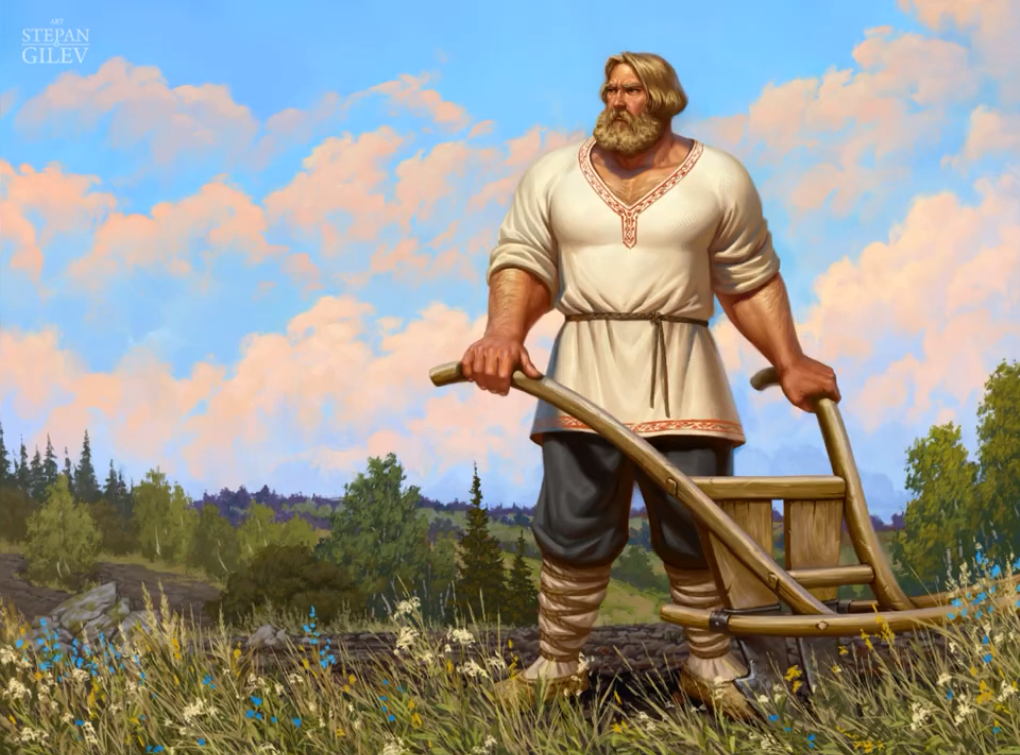
\includegraphics[scale=0.5]{img/plagiat}
        \caption{Отчет Антиплагиата}
        \label{fig:plagiat}
    \end{figure}
\end{center}

%\newpage
%\thispagestyle{empty}

%\vfill

\clearpage

\chapter*{Реферат}
\thispagestyle{plain}

Общий объем основного текста, без учета приложений ---
\pageref{end_of_main_text} страниц, с учетом приложений ---
22. Количество использованных источников~--- 9.
Количество приложений~--- 1.

%Ключевые слова:
Ключевые слова: ФАЗОВАЯ ДИАГРАММА, ВРЕМЕННОЙ РЯД, СТАЦИОНАРНОСТЬ, PYTHON

Целью работы является построение фазовых диаграмм временных рядов с использованием Python.

В первой части работы осуществляется теоретический анализ проблематики: рассматриваются основные компоненты
временных рядов и методы построения фазовых диаграмм. Акцентируется внимание на использовании Python
как инструмента для этих задач, включая обзор подходящих библиотек и инструментов программирования.

Вторая часть представляет собой практическое применение рассмотренных методов для лабораторной работы. Определяется основной подход к построению
фазовых диаграмм временных рядов в Python, который реализуется в виде программного кода. Описываются этапы
подготовки данных, построения фазовых диаграмм, корреляционного и спектрального анализа.


\clearpage

\tableofcontents{}

\clearpage

\chapter*{Введение}
\label{sec:afterwords}
\addcontentsline{toc}{chapter}{Введение}

\section*{Цель проекта}

Разработать и внедрить интегрированную систему для автоматизированного
отслеживания и представления статусов кабинетов НИЯУ МИФИ, путем создания
парсера для сбора актуальной информации о кабинетах с портала home.mephi и
разработки телеграмм-бота, который предоставляет удобный интерфейс
пользователям, исследующим наличие свободных аудиторий в реальном времени.

\section*{Функциональные требования}

\subsection*{a. Парсер:}
\begin{itemize}
    \item Автоматическое извлечение данных о кабинетах с портала home.mephi в
заданные интервалы времени.
    \item Сбор информации о расположении кабинетов, времени проведения занятий,
наличии проектора и другой необходимой информации.
    \item Обновление существующей базы данных новой информацией с сайта.
\end{itemize}

\subsection*{b. Телеграмм-бот:}
\begin{itemize}
    \item Интерактивный интерфейс для пользователей.
    \item Поиск свободных кабинетов в заданный период времени.
    \item Предоставление детализированной информации о кабинете (расположение,
наличие проектора и т. д.).
    \item Уведомления пользователю о статусе определенных кабинетов по запросу.
\end{itemize}

\section*{Инструментальные средства}

\begin{enumerate}
    \item \textbf{Draw.io:} Инструментальное средство для визуализации диаграмм,
предоставляющее возможности отображения архитектурных решений, процессов и
компонентного взаимодействия.
    \item \textbf{Golang (Go):} Эффективный язык программирования с
характеристиками высокой производительности, подходящий для разработки парсеров
в связи с способностью обрабатывать значительные объемы данных.
    \item \textbf{PostgreSQL на CleverCloud:} Облачная реализация базы данных
PostgreSQL обеспечивает устойчивость, защиту данных и масштабируемость,
минимизируя задачи администрирования.
    \item \textbf{Yandex Cloud:} Облачная инфраструктура, включающая в себя:
    \begin{enumerate}[\alph{enumii}.]
        \item \textbf{Yandex Cloud Functions:} Serverless-технология для
исполнения кода в ответ на события, исключающая необходимость серверного
администрирования.
        \item \textbf{Yandex API Gateway:} Средство управления входящими
API-запросами с функционалом безопасности и маршрутизации.
        \item \textbf{Yandex Message Queue:} Сервис для асинхронного обмена
сообщениями, подходящий для задач межкомпонентного взаимодействия.
    \end{enumerate}
    \item \textbf{IDE (Goland, Datagrip):} 
    \begin{itemize}
        \item Goland: Интегрированная среда разработки, оптимизированная для
языка Go.
        \item Datagrip: Инструмент для работы с базами данных, в т.ч.
PostgreSQL.
    \end{itemize}
    \item \textbf{GitHub:} Платформа для хранения и версионного контроля
исходного кода, предоставляющая инструменты для коллаборативной разработки.
\end{enumerate}

\clearpage

\chapter{Архитектура системы}

\begin{figure}[h]
    \centering
    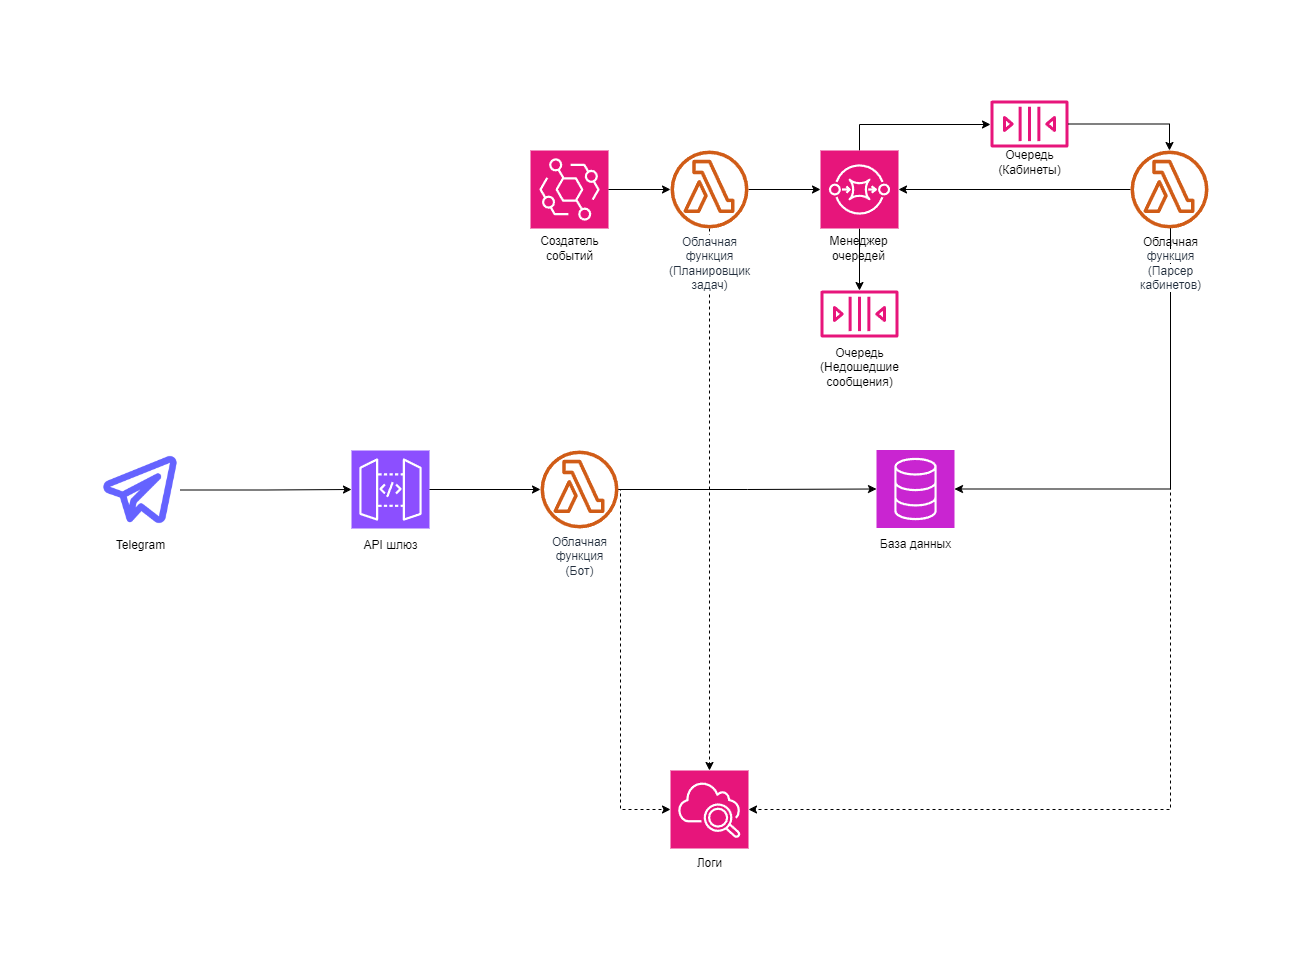
\includegraphics[scale=0.4]{img/functional}
    \caption{Архитектура системы}
    \label{fig:cp}
\end{figure}

\begin{enumerate}
    \item \textbf{Telegram}: Это мессенджер, с которым пользователи
взаимодействуют для отправки и получения сообщений.
    
    \item \textbf{API Шлюз}: Этот компонент обеспечивает взаимодействие между
Telegram и основной функциональностью бота. Он служит мостом для передачи данных
между мессенджером и другими компонентами системы.
    
    \item \textbf{Облачная функция (Бот)}: Центральная часть системы, которая
обрабатывает запросы пользователей и взаимодействует с другими частями системы.
Отсюда отправляются запросы к менеджеру операций, парсеру кабинетов и базе
данных.
    
    \item \textbf{Создатель событий}: Этот компонент генерирует определенные
события или уведомления для менеджера операций.
    
    \item \textbf{Менеджер операций}: Обрабатывает запросы от облачной функции и
координирует выполнение различных операций (выполняет роль автоматического
создателя задач парсеру, т.е какую информацию необходимо собрать с home.mephi).
Также взаимодействует с очередями сообщений.
    
    \item \textbf{Очередь (Кабинеты)}: Хранит информацию о задачах или запросах,
ожидающих выполнения.
    
    \item \textbf{Очередь (Неотвеченные сообщения)}: Хранит информацию о
сообщениях или запросах, на которые еще не был дан ответ в следствие ошибки.
    
    \item \textbf{Облачная функция (Парсер кабинетов)}: Анализирует и
обрабатывает информацию о различных кабинетах с home.mephi.
    
    \item \textbf{База данных}: Хранилище всей информации, необходимой для
работы системы.
    
    \item \textbf{Логи}: Записи о всех операциях и событиях, происходящих в
системе.
\end{enumerate}


\chapter{Выбор модели жизненного цикла}

В контексте рассматриваемого проекта принято решение применять
Agile-методологию. Выбор данной методологии обусловлен следующими причинами:

\begin{enumerate}
    \item \textbf{Динамичность требований.} Agile ориентирован на проекты с
переменчивыми требованиями, что обеспечивает возможность адаптации команды к
обновленным условиям или к обратной связи от стейкхолдеров.
    
    \item \textbf{Оперативная обратная связь.} Основной фокус Agile -- получение
регулярной обратной связи, что способствует раннему обнаружению и решению
проблем, а также проверке соответствия решения ожиданиям заказчика.
    
    \item \textbf{Регулярное обновление продукта.} Agile предполагает частое
внедрение нового функционала, позволяя конечным пользователям активно
тестировать систему и предоставлять свои отзывы.
    
    \item \textbf{Адаптивность.} В условиях переменчивости контекста, как,
например, изменения на web-портале home.mephi, Agile обеспечивает способность
команды к гибкому реагированию.
    
    \item \textbf{Коллаборация.} Agile ставит акцент на совместной работе
разработчиков, заказчика и других участников, создавая прозрачную среду и
атмосферу доверия.
    
    \item \textbf{Ориентированность на пользователя.} В разработке систем с
пользовательским интерфейсом, таких как телеграмм-бот, первостепенное значение
имеет учет требований и потребностей конечного пользователя.
    
    \item \textbf{Мониторинг рисков.} Регулярные итерации и постоянная оценка
позволяют эффективно идентифицировать и контролировать потенциальные риски
проекта.
\end{enumerate}

Учитывая указанные аргументы, применение Agile-методологии для данного проекта
является обоснованным выбором.

\clearpage

\chapter{Диаграмма прецедентов}

\begin{figure}[h]
    \centering
    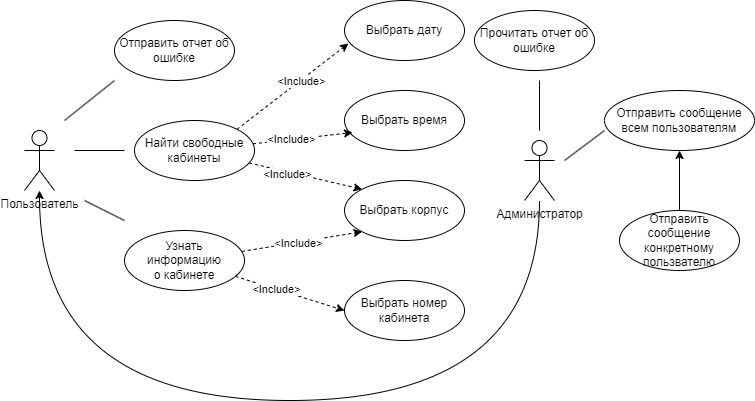
\includegraphics[scale=0.6]{img/prec}
    \caption{Диаграмма прецедентов}
    \label{fig:cp}
\end{figure}

Актеры:

Пользователь: Основной пользователь системы. Его действия в системе направлены
на получение информации о кабинетах.
Администратор: Ответственный за управление системой. Его функции включают в себя
прочтение отчетов об ошибках и отправку сообщений пользователям.

Прецеденты Пользователя:

Узнать информацию о кабинете: Пользователь может запросить информацию о
конкретном кабинете. Для этого ему потребуются следующие дополнительные
действия:

Выбрать корпус: Пользователь выбирает интересующий его корпус.

Выбрать номер кабинета: После выбора корпуса, пользователь указывает номер
интересующего его кабинета.

Аналогично пользователь может получить список свободных кабинетов, введя дату и
время.

Отправить отчет об ошибке: Если пользователь обнаружил ошибку в информации или в
работе системы, он может отправить отчет администратору.

Прецеденты Администратора:

Прочитать отчет об ошибке: Администратор имеет возможность просмотреть
полученные отчеты об ошибках от пользователей.

Отправить сообщение всем пользователям: В случае необходимости администратор
может отправить сообщение всем пользователям системы.

Отправить сообщение конкретному пользователю: Администратор может направить
сообщение определенному пользователю, например, чтобы уточнить детали отчета об
ошибке или предоставить индивидуальную информацию.

Отношения между прецедентами:
Администратор может выполнять все функции, доступные пользователю.

\chapter{Карта сайта}

\begin{figure}[h]
    \centering
    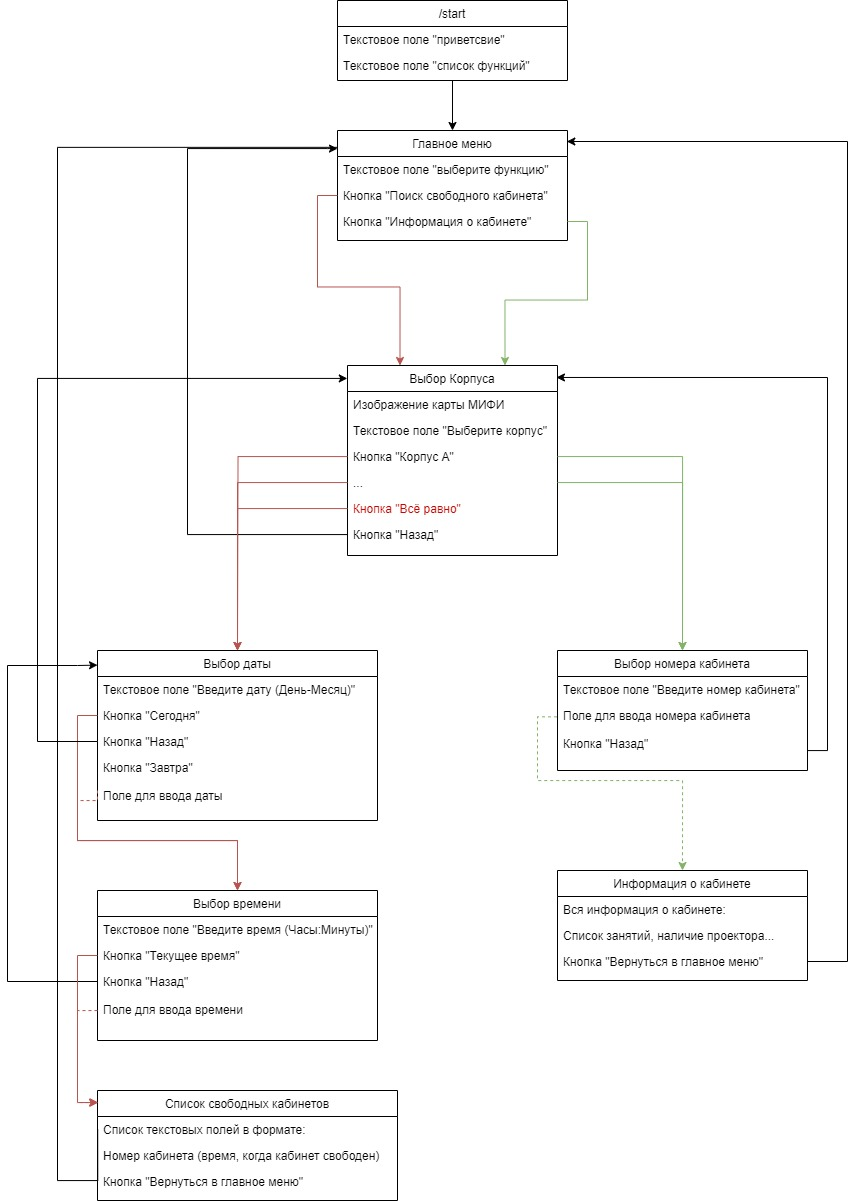
\includegraphics[scale=0.45]{img/map}
    \caption{Карта сайта}
    \label{fig:cp}
\end{figure}

1. Стартовое меню:

При запуске бота пользователь видит приветственное сообщение и список доступных
функций:

Поиск свободного кабинета

Информация о кабинете

Пользователь может выбрать одну из предложенных функций, нажав соответствующую
кнопку.

2. Выбор корпуса:

При выборе поиска свободного кабинета пользователь должен указать корпус здания,
в котором будет произведен
поиск (существует опция поиска по всем корпусам) либо вернуться в главное меню.
Для удобства пользователя бот покажет карту университета.

3. Выбор даты:

Пользователь вводит дату в формате (День-Месяц), либо может вернуться на
предыдущий этап.

Для удобства пользователя всплывают кнопки:
"Сегодня": При выборе этой кнопки поиск будет проводиться на текущую дату.
"Завтра": При выборе этой кнопки поиск будет проводиться на следующий день.

4. Выбор времени:

После выбора даты пользователь указывает время в формате (Часы:Минуты), либо
может вернуться на предыдущий этап.

Для удобства пользователя всплывает кнопка:
"Текущее время": При выборе этой кнопки поиск будет проводиться на текущее
время.

5. Список свободных кабинетов:

После ввода всех параметров пользователю выводится список свободных кабинетов:

Список текстовых полей: Каждое поле содержит информацию о свободном кабинете
(номер кабинета, интервал времени, когда кабинет освободится).
Также появится кнопка "Вернуться в главное меню".

6. Выбор номера кабинета:

Если пользователь хочет узнать информацию о конкретном кабинете, то после выбора
корпуса
ему необходимо ввести номер желаемого кабинета.

7. Информация о кабинете:

Вся информация о кабинете: Список занятий, наличие проектора и др.
Также появится кнопка "Вернуться в главное меню": Возврат в главное меню.

\chapter{Схема базы данных}

Данная система должна хранить в себе следующие данные:
\begin{itemize}
    \item Информацию о аудиториях в НИЯУ МИФИ, включая их характеристики, такие
как наличие проектора, компьютера...
    \item Данные о пользователях системы.
    \item Подробности о занятиях, такие как их тип, предмет, время начала и
окончания, дни проведения, семестр и аудитория.
    \item Информацию о преподавателях, включая их короткие имена или инициалы.
    \item Сведения о студенческих группах.
\end{itemize}

Можно заметить, что данные, которые необходимо хранить, обладают четкой
структурой и имеют связи. Например, каждый урок связан с конкретной аудиторией и
может быть связан с несколькими преподавателями или студенческими группами. Эти
связи помогут в организации расписания и оптимизации использования ресурсов
учебного заведения.

Важными факторами при выборе системы управления базы данных являются:
\begin{itemize}
    \item Производительность: Система должна быстро обрабатывать запросы и
обеспечивать минимальные задержки при работе с большим объемом данных.
    \item Масштабируемость: Возможность расширения системы для работы с
увеличивающимся объемом данных без значительного снижения производительности.
    \item Надежность: Гарантия сохранности данных даже при возникновении
технических сбоев.
    \item Безопасность: Защита данных от несанкционированного доступа и утечек.
    \item Поддержка: Наличие обширной документации, сообщества пользователей и
профессиональной технической поддержки.
\end{itemize}

\begin{figure}[h]
    \centering
    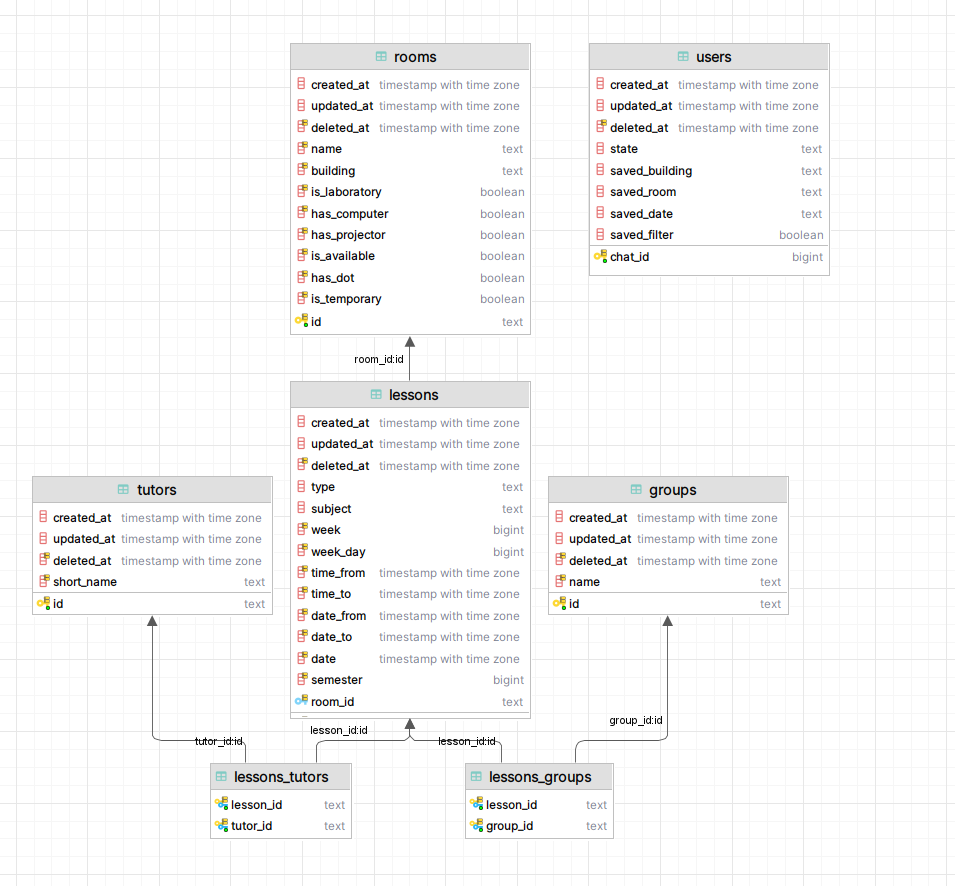
\includegraphics[scale=0.6]{img/bd}
    \caption{Схема базы данных}
    \label{fig:cp}
\end{figure}


\subsection*{1. Таблица ``rooms'' (Кабинеты):}
Эта таблица содержит информацию о аудиториях в НИЯУ МИФИ.
\begin{itemize}
    \item \textbf{created\_at, updated\_at, deleted\_at}: Даты создания,
обновления и удаления записи.
    \item \textbf{name}: Название аудитории.
    \item \textbf{building}: Здание, в котором находится аудитория.
    \item \textbf{is\_laboratory}: Флаг, указывающий, является ли аудитория
лабораторией.
    \item \textbf{has\_computer, has\_projector}: Флаги, указывающие на наличие
компьютера и проектора в аудитории.
    \item \textbf{is\_available}: Доступность аудитории.
    \item \textbf{has\_dot, is\_temporary}: Дополнительные характеристики
аудитории (ДОТ, выездная аудитория).
    \item \textbf{id}: Уникальный идентификатор аудитории.
\end{itemize}

\subsection*{2. Таблица ``users'' (Пользователи):}
Содержит информацию о пользователях системы.
\begin{itemize}
    \item \textbf{created\_at, updated\_at, deleted\_at}: Даты создания,
обновления и удаления записи.
    \item \textbf{state}: Состояние пользователя.
    \item \textbf{saved\_building, saved\_room, saved\_date}: Сохраненный запрос
пользователя (здание, комната и дата).
    \item \textbf{saved\_filter}: Сохраненный запрос пользователя (наличие
проектора в аудитории).
    \item \textbf{chatId}: Идентификатор чата пользователя в Telegram.
\end{itemize}

\subsection*{3. Таблица ``lessons'' (Уроки):}
Информация о уроках или занятиях.
\begin{itemize}
    \item \textbf{created\_at, updated\_at, deleted\_at}: Даты создания,
обновления и удаления записи.
    \item \textbf{type, subject}: Тип(Лек, Пр...) и название предмета.
    \item \textbf{week, week\_day}: Неделя и день недели пары.
    \item \textbf{time\_from, time\_to}: Время начала и окончания пары.
    \item \textbf{date\_from, date\_to}: Даты начала и окончания пары.
    \item \textbf{semester}: Семестр.
    \item \textbf{room\_id}: Идентификатор комнаты, в которой проводится урок.
\end{itemize}

\subsection*{4. Таблица ``tutors'' (Преподаватели):}
Информация о преподавателях.
\begin{itemize}
    \item \textbf{created\_at, updated\_at, deleted\_at}: Даты создания,
обновления и удаления записи.
    \item \textbf{short\_name}: Инициалы преподавателя.
    \item \textbf{id}: Уникальный идентификатор преподавателя.
\end{itemize}

\subsection*{5. Таблица ``groups'' (Группы):}
Содержит информацию о студенческих группах.
\begin{itemize}
    \item \textbf{created\_at, updated\_at, deleted\_at}: Даты создания,
обновления и удаления записи.
    \item \textbf{name}: Название группы.
    \item \textbf{id}: Уникальный идентификатор группы.
\end{itemize}

\subsection*{6. Таблица ``lessons\_tutors'' (Пары и преподаватели):}
Связывает пары с преподавателями.
\begin{itemize}
    \item \textbf{lesson\_id, tutor\_id}: Идентификаторы урока и преподавателя.
\end{itemize}

\subsection*{7. Таблица ``lessons\_groups'' (Пары и группы):}
Связывает пары со студенческими группами.
\begin{itemize}
    \item \textbf{lesson\_id, group\_id}: Идентификаторы урока и группы.
\end{itemize}

\clearpage

\chapter{Основные сценарии использования системы}

\section*{Сценарии}

\subsection*{1. Поиск свободной аудитории}
\textbf{Предусловие:} Пользователь открыл телеграмм-бот.

\begin{enumerate}
    \item Пользователь вводит параметры поиска (например, время, вместимость
аудитории, наличие проектора).
    \item Система обращается к базе данных и ищет соответствующие свободные
аудитории.
    \item Система выводит пользователю список подходящих аудиторий.
    \item Пользователь может выбрать конкретную аудиторию для просмотра более
подробной информации.
\end{enumerate}

\subsection*{2. Просмотр расписания аудитории}
\textbf{Предусловие:} Пользователь находится в интерфейсе телеграмм-бота.

\begin{enumerate}
    \item Пользователь выбирает интересующую его аудиторию.
    \item Система извлекает и выводит текущее расписание для выбранной
аудитории.
\end{enumerate}

\subsection*{3. Автоматическое обновление информации о аудиториях}
\textbf{Предусловие:} На сайте home.mephi появилась обновленная информация о
кабинетах.

\begin{enumerate}
    \item По заданному расписанию или триггеру парсер начинает процесс
обновления данных.
    \item Парсер собирает актуальную информацию с сайта home.mephi.
    \item Обновленные данные записываются в базу данных.
    \item Если в процессе возникли ошибки, система отправляет уведомления
системному администратору.
\end{enumerate}

\chapter{Диаграммы последовательностей}

Поиск свободных кабинетов:
\begin{figure}[h]
    \centering
    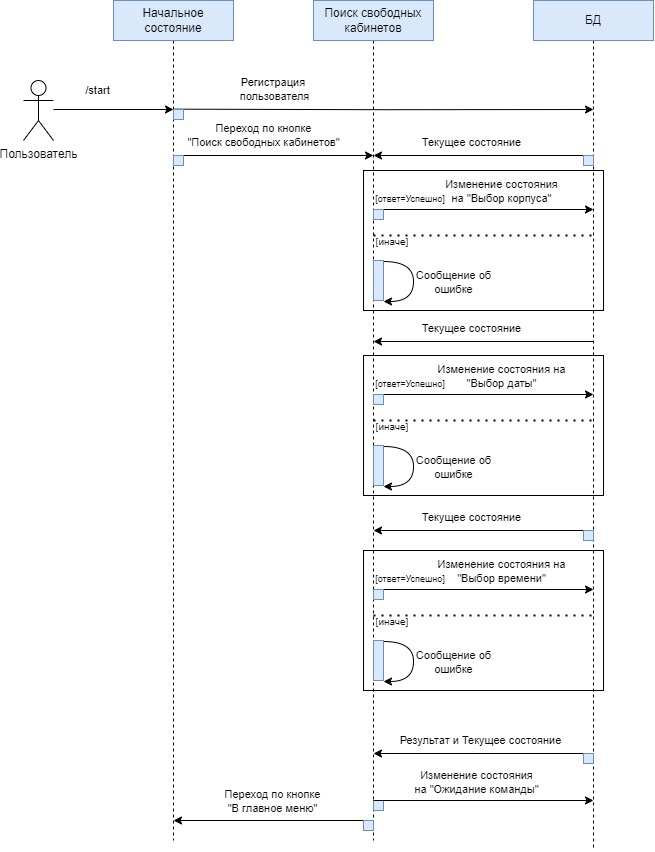
\includegraphics[scale=0.6]{img/seq1}
    \caption{диаграмма последовательности}
    \label{fig:cp}
\end{figure}

Получение информации о кабинете:
\begin{figure}[h]
    \centering
    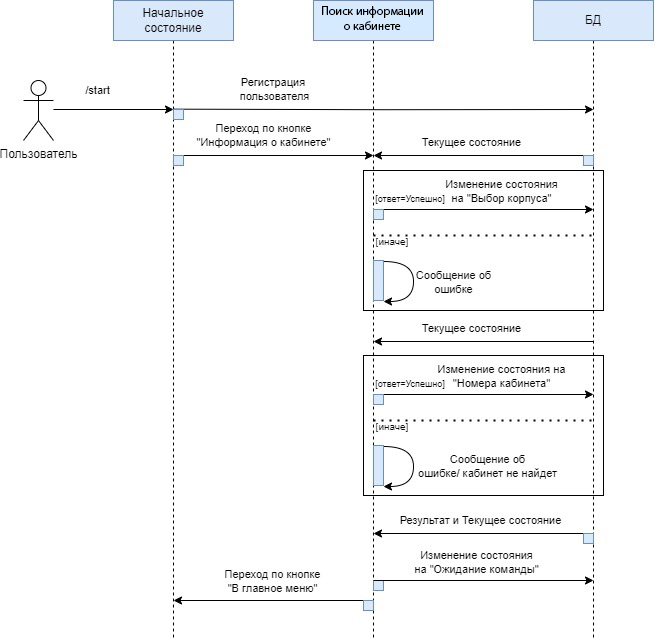
\includegraphics[scale=0.6]{img/seq2}
    \caption{диаграмма последовательности}
    \label{fig:cp}
\end{figure}

\clearpage

\chapter{Руководство пользователя для системы}

\section*{Введение}

Система предназначена для автоматизированного отслеживания и представления
статусов кабинетов НИЯУ МИФИ. Это руководство поможет вам ознакомиться с
функциональностью телеграмм-бота системы.

\section*{Начало работы}

\subsection*{Доступ к боту}
Для начала работы откройте Telegram и найдите бота по названию
\texttt{@}mephi\_checker\_bot. Нажмите на ``Старт'' для инициализации бота.

\begin{figure}[h]
    \centering
    
\includegraphics[scale=0.8]{img/1}
    \caption{}
    \label{fig:cp}
\end{figure}

\section*{Основные функции}
\begin{enumerate}
    \item Поиск свободных аудиторий
    \item Информация о конкретной аудитории
\end{enumerate}

\section*{Поиск свободных аудиторий}
Сначала необходимо выбрать корпус, в котором будет происходить поиск:
\begin{figure}[h]
    \centering
    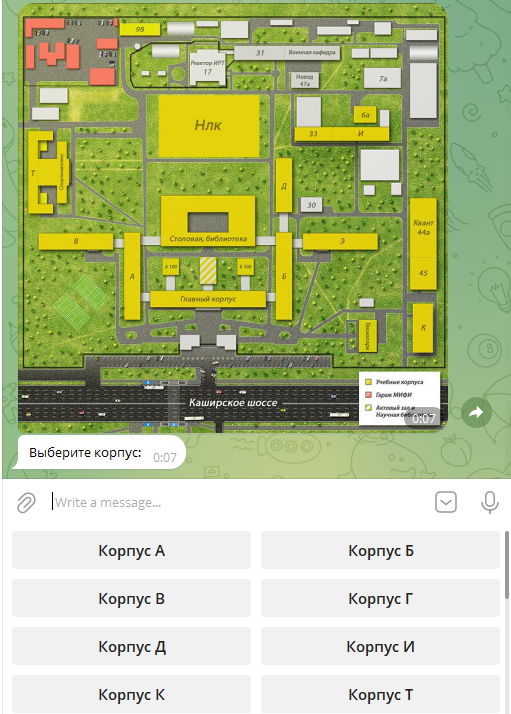
\includegraphics[scale=0.8]{img/2}
    \caption{Интерфейс бота(карта кабинета)}
    \label{fig:cp}
\end{figure}

После этого необходимо ввести дату поиска:
\begin{figure}[h]
    \centering
    
\includegraphics[scale=0.8]{img/3}
    \caption{Интерфейс бота(ввод даты)}
    \label{fig:cp}
\end{figure}

Последним этапом является ввод времени поиска:
\begin{figure}[h]
    \centering
    
\includegraphics[scale=0.8]{img/4}
    \caption{Интерфейс бота(ввод времени)}
    \label{fig:cp}
\end{figure}

В результате пользователь получит список свободных кабинетов с
интервалом времени, когда он может его занять:
\begin{figure}[h]
    \centering
    
\includegraphics[scale=0.8]{img/5}
    \caption{Интерфейс бота(результат поиска)}
    \label{fig:cp}
\end{figure}

\section*{Информация о конкретной аудитории}
Сначала необходимо выбрать корпус, в котором будет происходить поиск:
\begin{figure}[h]
    \centering
    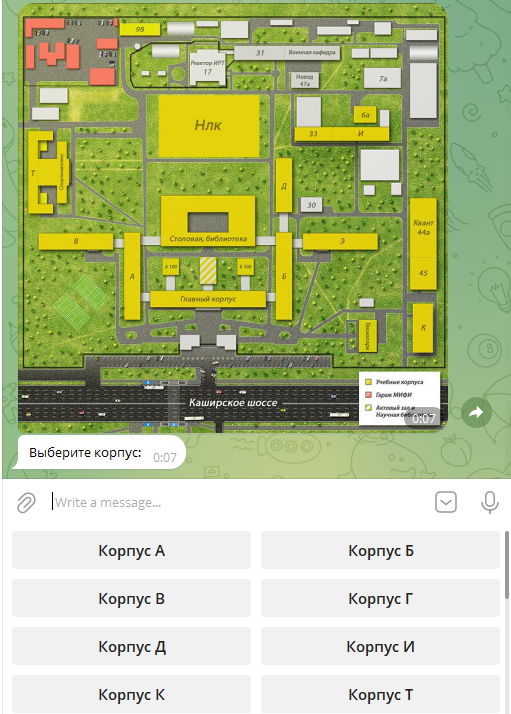
\includegraphics[scale=0.8]{img/2}
    \caption{Интерфейс бота(карта кабинета)}
    \label{fig:cp}
\end{figure}

После этого необходимо номер кабинета:
\begin{figure}[h]
    \centering
    
\includegraphics[scale=0.8]{img/6}
    \caption{Интерфейс бота(ввод номера кабинета)}
    \label{fig:cp}
\end{figure}


В результате пользователь получит полную информацию о кабинете:
\begin{figure}[h]
    \centering
    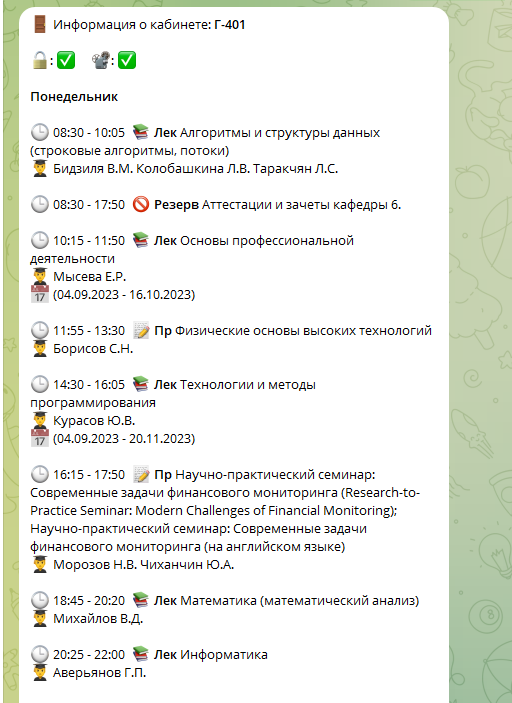
\includegraphics[scale=0.8]{img/7}
    \caption{Интерфейс бота(результат)}
    \label{fig:cp}
\end{figure}


\clearpage

\chapter*{Заключение}
\addcontentsline{toc}{chapter}{Заключение}

В ходе выполнения данной учебно-исследовательской работы было проведено
исследование инструментов развертывания контейнеризированных сред и возможностей
их интеграции с Terraform и Scala. Был проведен анализ системы Kubernetes и её
особенностей типизации, а также исследованы возможности интеграции системы
Kubernetes с Terraform. Было проведено сравнение различных систем, таких как
k3s, Kubernetes и Minikube.

В результате анализа была разработана алгебраическая модель для представления
определений Terraform, включая определение основных типов и структур данных, а
также функций для обработки и развертывания определений Terraform.

Была спроектирована архитектура модуля-обертки для развертывания типизированных
определений Terraform, включая разработку интерфейсов и классов модуля для
генерации HCL конфигурации, а также функций для взаимодействия с Kubernetes и
Terraform.

В ходе реализации был создан парсер для плагинов Terraform, парсер документации,
а также модуль Case Classes Generator. Был реализован модуль для работы с
Kubernetes API.

Однако, несмотря на значительные успехи, работа над проектом еще не завершена.
Некоторые из модулей, описанных в разделе 3, еще требуют реализации. Это
подчеркивает сложность и масштаб задачи, а также необходимость продолжения
работы над проектом.

В целом, проделанная работа демонстрирует возможность интеграции системы
Terraform с Scala и Kubernetes, что открывает новые возможности для
автоматизации и оптимизации процессов развертывания и масштабирования
приложений. Однако, для достижения полной функциональности и надежности,
необходимо продолжить разработку и тестирование оставшихся модулей.


\label{end_of_main_text}

\setcounter{totalfigures}{\the\value{totalfigures}+\the\value{figure}}
\setcounter{figure}{0}
\setcounter{totaltables}{\the\value{totaltables}+\the\value{table}}
\setcounter{table}{0}
\setcounter{totallistings}{\the\value{totallistings}+\the\value{lstlisting}}
\setcounter{lstlisting}{0}

\makeatletter
\edef\@currentlabel{\the\value{totalfigures}}
\label{figures}
\edef\@currentlabel{\the\value{totaltables}}
\label{tables}
\edef\@currentlabel{\the\value{totallistings}}
\label{listings}
\makeatother

\clearpage

\sloppy

\phantomsection
\addcontentsline{toc}{chapter}{\bibname}	% Добавляем список литературы в оглавление
\printbibliography
% печать библиографии через BibLaTeX

\fussy

% \addcontentsline{toc}{section}{Список литературы}
% \begin{thebibliography}{99}


% %\bibitem{RCO1} {Ермаков А.Е.  Автоматизация онтологического инжиниринга в системах извлечения знаний из текста. М.: ООО ``ЭР СИ О'', Компьютерная лингвистика и интеллектуальные технологии: труды Международной конференци Диалог'2008, 2008.}


% %\bibitem{Troel} {Троелсен Э. Язык программирования C\# 2008  и платформа .Net 3.5  М.: издательство <<Вильямс>>{}, 2010. 1344 с.}


% %\bibitem{PBIRCH}{Ashwani Garg, Ashish Mangla, Neelima Gupta, Vasudha Bhatnagar PBIRCH: A scalable parallel clustering algorithm for incremental data. //Proceedings of 10th International Database Engineering and Applications Symposium IDEAS06, 2006}



% \end{thebibliography}


\endrefsection

\clearpage

% \chapter*{Приложения}
%\addcontentsline{toc}{chapter}{Приложения}
%\appendixtocon
%\renewcommand{\appendixname}{Приложение}
\appendix
\renewcommand{\appendixtocname}{Приложения}
\addappheadtotoc
%\titleformat{\chapter}[block]{\centering\normalfont\Large\bfseries}{\chaptername{} \thechapter.}{1ex}{}{}
\renewcommand{\chaptername}{Приложение}
%\renewcommand*\printchaptername{\Large\bfseries\appendixname~}
%\renewcommand{\thechapter}{Приложение \Alph{chapter}}
%\renewcommand{\thechaptertoc}{Приложение \Alph{chapter}}

%\renewcommand{\chaptermark}[1]{\markboth{\chaptername\ \thechapter.\ #1}{}}

\begin{appendices}

\chapter{Пример кода парсера terraform plugin}\label{sec:appendix1}
%\addcontentsline{toc}{chapter}{}

\begin{lstlisting}[language=Go]
package main

import (
"encoding/json"
"github.com/terraform-providers/terraform-provider-aws/aws"
"os"
"reflect"
)

// Функции для обработки различных типов значений

func processValue(value reflect.Value) (interface{}, bool) {
// ...
}
func walkStruct(v reflect.Value) map[string]interface{} {
// ...
}
func walkSlice(v reflect.Value) []interface{} {
// ...
}
func walkMap(v reflect.Value) map[string]interface{} {
// ...
}
func valueIsValid(value reflect.Value) bool {
// ...
}

func check(e error) {
if e != nil {
panic(e)
}
}

func main() {
// Инициализация плагина
provider := aws.Provider()

// Извлечение информации о провайдере
providerValue := reflect.ValueOf(provider).Elem()
providerInfo := walkStruct(providerValue)

// Конвертация информации о провайдере в JSON
m, err := json.MarshalIndent(providerInfo, "", "  ")
check(err)

// Сохранение JSON в файл
err = os.WriteFile("./aws.json", m, 0644)
check(err)
}
\end{lstlisting}

\clearpage

% \input{chapters/thesis-template-appendix2.tex}

% \clearpage

% \input{chapters/thesis-template-appendix3.tex}

% \clearpage

% \input{chapters/thesis-template-appendix4.tex}

% \clearpage

% \input{chapters/thesis-template-appendix5.tex}

% \clearpage

% \input{chapters/thesis-template-appendix6.tex}

\end{appendices}

\label{end_of_document}


\end{document}
